\documentclass{article}
\usepackage{graphicx} % Required for inserting images
\usepackage{url}
\usepackage{tikz}
\usepackage{hyperref}

\graphicspath{{./diagram/}}

% \title{Thesis Proposal}

\author{Navid Rahimidanesh}
\date{March 2023}

\begin{document}

% \maketitle

\begin{titlepage}
    \begin{center}
        \vspace*{1cm}
        
        \huge
        \textbf{Thesis Proposal}
        
        \vspace{0.5cm}
        \LARGE
        Towards a Data Space for Collaborative Cyber Threat Intelligence Sharing
        
        \vspace{1.5cm}
        
        \textbf{Navid Rahimidanesh}
        
        \vfill
        
        A thesis presented for the degree of\\
        Master of Science
        
        \vspace{0.8cm}
        
        % \includegraphics[width=0.4\textwidth]{logo}
        
        \Large
        Department of Computer Science\\
        University of RWTH\\
        Germany\\
        \today
        
    \end{center}
\end{titlepage}

\tableofcontents

\newpage

\section{Abstract}

TODO

\section{Introduction} % 1.5 Page

\subsection{Motivation}

% - Why is it important?
% - High level description of the problem
% - Real world


% - CTI

Cyber threat intelligence (CTI) refers to all  information that that can help an organization identify, assess, and respond to cyber threats. It includes information about threat actors, their motivations, tactics, techniques, and procedures (TTPs), indicators of compromise (IOCs), the systems' vulnerabilities, incident response plans and mitigation strategies. A structured CTI program is crucial for a comprehensive cybersecurity strategy.
To be one step ahead of the attacker, organizations often share the CTI they have gathered with each other. This is called collaborative CTI (CCTI). 

% - CCTI

However, there are several challenges for CCTI: Firstly, this information is potentially confidential. Adversaries can perform attack using the same techniques mentioned in the CTI. Thus, forming the necessary trust relationship is a challenge that keeps the sharing so limited. Secondly, due to the criticality of the information there are regulations further limiting the sharing. For example, the General Data Protection Regulation (GDPR) limits the transfer of personal data outside the EU. Thirdly, the lack of a standardized format for CTI is another challenge.

% - Data Spaces

Some of these challenges could be addressed by data sovereignty, which is the ability of the data owner to control what happens to the data after it is shared. There are efforts to standardize a data exchange scheme that enables data sovereignty. Gaia-X and International Data Spaces (IDS) are two examples. These projects are getting more popularity, therefore it is important to investigate their potentials and limitations. As far as my knowledge, there is no work that has investigated the potentials of data spaces in the context of CTI sharing. 


\subsection{Thesis Goal}

% Towards CTI Data space.
% Identify capabilities and limitations.
% Define guidelines and provide recommendations.

% Reference Architecture
% Standards
% 

This thesis aims to explore the efficacy of leveraging data spaces in the domain of Cyber Threat Intelligence (CTI) sharing. The primary objective is to design, implement, and evaluate a prototype data space tailored for CTI sharing. By delving into established data space methodologies, with a specific emphasis on International Data Spaces (IDS), the research will contribute insights into their potential applications within the realm of cybersecurity.

The research will also investigate the current landscape of cybersecurity in smart grids to identify a pertinent use case for the developed prototype. This multifaceted approach seeks to achieve four main contributions:

\begin{enumerate}
    \item 
    \textbf{Exploration of Data Space Potential:} Investigating the viability of international data spaces for enhancing the sharing of Cyber Threat Intelligence.

    \item
    \textbf{Architectural Design and Prototype Implementation:} Developing a sample architecture and specific standards for data spaces in the context of CTI sharing and realizing it through the implementation of a prototype.
    
    \item
    \textbf{Concrete Use Case Extraction:} Identifying and illustrating a specific use case scenario for the proposed platform within the domain of smart grids.
    
    \item
    \textbf{Evaluation and Limitation Identification:} Assessing the performance of the prototype and delineating its limitations, providing valuable insights for future improvements and iterations.
\end{enumerate}


Through this comprehensive investigation, the thesis aims to contribute to the advancement of collaborative CTI efforts by harnessing the potential of data spaces while addressing the intricacies and challenges associated with CTI sharing in the cybersecurity landscape.
\subsection{Outline}

The rest of the thesis is structured as follows: Section \ref{sec:background} provides the necessary background information. Section \ref{sec:related-work} reviews the related work. Section \ref{sec:use-case} describes the use case and the requirements. Section \ref{sec:conceptual-approach} describes the conceptual approach. Section \ref{sec:realization} describes the conceptual approach. Section \ref{sec:evaluation} describes how the evaluation should be. Section \ref{sec:timeline} describes the timeline and plan.

\section{Background} % 4 pages
\label{sec:background}
In this section, we will review the relevant concepts and technologies that are necessary to understand the rest of the work.

\subsection{Cybersecurity}
% TODO: Use references for Definitions

Cybersecurity, the practice of protecting computer systems, networks, and data, encompasses crucial terms such as confidentiality, ensuring data privacy; integrity, maintaining data accuracy and trustworthiness; availability, assuring data and systems are accessible when needed; authentication, verifying user identities; authorization, granting appropriate access; firewall, filtering network traffic; malware, malicious software; phishing, deceptive attacks; and vulnerability, weaknesses in systems.


Relevant actors in the realm of cybersecurity include hackers who exploit vulnerabilities, security analysts responsible for defending systems, vendors who create security solutions, employees who can pose potential insider threats, government bodies serving as regulators and law enforcement, threat actors with malicious intent, and end users utilizing digital resources in the interconnected digital landscape.

\subsection{Cyber Threat Intelligence}
Cyber threat intelligence (CTI) is the process of collecting, analyzing, and disseminating information about potential or current cyber threats. CTI relies on gathering data from diverse sources, including security tools, threat feeds, honeypots, forums, social media platforms, and other relevant online and offline sources. This data can include indicators of compromise (IOCs), malware samples, network traffic logs, vulnerability information, and more. The goal is to provide organizations with a comprehensive understanding of potential cyber threats to make informed decisions. It helps identify the tactics, techniques, and procedures (TTPs) used by threat actors and vulnerabilities in an organization's security infrastructure. It is an important component of a comprehensive cybersecurity strategy to reduce the risk of a cyberattack. 

% Threat Intelligence Program
    % Threat Intelligence Cycle: Planning / Collection / Analysis / Production / Dissemination
% Situational Awareness (SA)
% TTPs
% Threat Actors
% Vulnerabilities
% IOCs
    % Malware
% Incident Response (IR)
    % Playbook
% General Recommendations
    % Risk mitigation strategies


\subsection{Collaborative CTI} \label{sec:ccti}

CTI can be collaborative, meaning it can involve multiple organizations with a common goal.
By sharing CTI, stakeholders can gain a better understanding of the threat landscape and a wider situational awareness. 
This can help them identify and proactively mitigate threats instead of reacting to them after they have occurred.
Plus, security teams reduce their workload by not doing the same thing that has already been done by others. As a result, they can focus on investigating unknown threats. 
Moreover, it is common for a threat actor to target multiple organizations using the same TTPs, because once an attack vector is successful, the attacker will try to exploit using it as much as possible, further increasing the benefits of CTI sharing.
However, for an effective CTI sharing, CTI should be timely and actionable. 
Constantly, the vulnerabilities get patched, malwares gets updated, and threat actors change their TTPs. Therefore, CTI should be shared in real-time to be most effective. 
Furthermore, CTI should be actionable, meaning the receiving organization should be able to easily turn it into actions. Should it take a lot of effort to process the CTI, it will waste security team's resources.
These points suggest the importance of automation in CTI sharing.

There are existing frameworks and communities for CTI sharing. Information Sharing and Analysis Centers (ISACs) are one. These are non-profit organizations that help organizations in a specific sector, usually a critical national infrastructure, e.g. electricity, water, gas, health care, finance, etc., to share CTI with each other. 

Despite the benefits of CTI sharing, there are also gaps and limitations that need to be addressed. 
These include concerns around market factors, legal and regulatory barriers, lack of trust among participants, and interoperability challenges.
% Market
Organizations fear that sharing CTI will expose their vulnerabilities and in turn cause negative publicity.
% Legal and Liability
Liability is another concern. Third party tools whose vulnerabilities are shared through CTI might sue the organization that shared the information. Personal data protection laws, such as GDPR, should be considered when sharing CTI.
% Trust
Many CTI sharing communities suffer from free-riding--where some organizations benefit from the shared CTI without contributing any CTI of their own. 
Another concern is the risk of hackers gaining access to the CTI. 
% Interoperability
The lack of a standardized format for CTI is another challenge. Each organization uses its own chosen format to consume and manage CTI, therefore the CTI provider should produce CTI in many formats.
% Effort and Benefit
A CTI provider should consider all these challenges before sharing CTI, which might require a lot of resources and many skilled personnel costing the organization a lot of money.

\paragraph{EE-ISAC}
An example ISAC would be
European Energy Information Sharing and Analysis Center (EE-ISAC)
which has acquired over 30 members from utilities, academia, governmental and non-governmental organizations since its foundation in 2015. Members exchange cyber threat information through plenary meetings, working groups, and a dedicated platform (based on MISP). The information exchange is based on a trust achieved by confidentiality agreements and regular physical meetings with the same members. 
\cite{wallis_ee-isacpractical_2022}


\paragraph{Obligatory Sharing}

The Directive on measures for a high common level of cybersecurity across the Union (the NIS2 Directive) provides legal measures to boost the overall level of cybersecurity in the EU. It ensures EU member states to have a national Computer Security Response Team (CSIRT) that cooperate with each other, and also a culture of information sharing between the public and private sectors in critical sectors. More specifically, organizations that are part of the critical sectors are required to share information about incidents happened to them with the national CSIRT.

% \subsection{Data Modeling}
% In the context of CTI sharing, data modelling serves three purposes: (1) to provide a backbone for all relevant information, (2) to specify the data input format for further analysis, (3) to define the desired target for information gathering. \cite{husak_crusoe_2022}

\subsection{Data Sovereignty}
By increasing the value of data in businesses and data becoming a commodity, protecting data using laws and regulations has become a necessity. Data sovereignty is concept that has arisen in this context. It refers to the right of the owner of the data to have control over their data. By default, if a party is processing data owned by another party, the processing party can technically do anything with the data. Data sovereignty tries to address this issue. One means of achieving data sovereignty is by using usage control. Usage control concerns with introducing and enforcing restrictions on what could (not) happen to the data. It is the generalized version of the traditional access control which only concerns with "who" rather than "how", "where", "why". The data owner defines the usage policies and the usage control mechanism enforces them. \cite{eitel_usage_2021}

\subsection{Data Spaces}
The term data spaces term was first coined by Franklin et al. \cite{franklin_databases_2005} to describe a new abstraction in data management to solve the data integration problem that follows: An organization has interrelated data in diverse origins, encompassing databases, files with various formats, and web services. The task is to query or update the data.
Franklin et al. proposed a DataSpace Suppport Platform (DSSP) that helps developers by providing a single query language based on a unified view of the data sources. This implies a pay-as-you-go approach where physically moving and transforming the data is done only by demand.

The same concept applies when several organizations want to integrate their data or exchange it with others. In this context, the term data space would refer to the platform comprised of data sources in different organizations used for data exchange and integration which is defined by a set of standards and protocols that enable interoperability between them. \cite{reiberg_what_2022}

\paragraph{Data Space Features}

Apart from data sharing and integration, data spaces can fulfill other requirements.
A crucial requirement, that makes data spaces interesting, is the sovereignty of data. Data spaces can fulfill data sovereignty by keeping the data in the owner's side, and only sharing the metadata publicly.
Another requirement is governance of the data space. In order to facilitate the cooperation of different participants, a set of policies, rules and protocols should exist. To define them, a governance body is commonly expected to exist \cite{reiberg_what_2022}.
Data spaces should be open, meaning anyone complying with the policies should be able to join, which encourages a fair and non-monopolistic market. This entails an easy access, which means, anyone should be able to connect with a limited effort.
Data spaces are usually designed to be decentralized and federated, meaning, there is no entity having direct control over all data exchanges. Different participants can interact with each other directly. This emphasizes the role of interoperability. This is only possible when certain open standards are established. Consequently, data spaces complying to the same standards can be embedded inside each other enabling cross-data-space exchange \cite{reiberg_what_2022}.

\noindent\fbox{%
    \parbox{\textwidth}{%
    "Data Spaces are defined as: A federated, open infrastructure for sovereign data sharing, based on common policies, rules and standards." \cite{reiberg_what_2022}
    }%
}

\subsection{Smart Grid Security}
% TODO: Improve using the new review paper
A smart grid is an advanced electrical grid that uses advanced technologies to efficiently manage the generation, distribution, and consumption of electricity. Smart grid security involves protecting the system from cybersecurity threats that can disrupt or damage the grid's operations. It can be divided into three layers: physical security, network security, and data security. Physical security includes measures to protect the physical infrastructure of the grid, such as substations, transformers, and power lines. This can include fencing, security cameras, and access controls. Network security involves protecting the communication networks used by the smart grid. This can include implementing firewalls, intrusion detection systems, and encryption to prevent unauthorized access or attacks. Data security involves protecting the data generated and used by the smart grid, including customer data, operational data, and control data. This can include implementing access controls, data encryption, and backup and recovery systems to ensure the availability and integrity of the data. 

Wallis et al. \cite{wallis_ee-isacpractical_2022} mentions the following severe cyber threats for smart grids and the energy sector in general: data injection attacks on state estimation \cite{deng_false_2019}, distributed denial of service (DDoS) and denial of service (DoS) attacks \cite{wang_coordinated_2019}, targeted attacks, coordinated attacks, hybrid attacks, and advanced persistent threats \cite{leszczyna_cybersecurity_2019}. Moreover, in recent years, ransomware campaigns have emerged as a significant risk to the sector \cite{keshavarzi_i2ce3_2020}.

% --------------------------------------------------------------
\section{Related Work}
\label{sec:related-work}

In this section, we will review some existing solutions related to our problem. 

\subsection{Existing CTI Sharing Platforms}

By the rise in the amount of CTI available, the need for tools to process them has increased. It lead to emergence of many Threat Intelligence Platforms (TIP). TIPs can fetch CTI from different repositories, process and correlate information, and visualize the results. They can also be used to collaborate and share CTI with other organizations who use the same platform.

\paragraph{Proprietary TIPs} 
There are paid services that provide curated CTI feeds and more complex dashboards. There are many proprietary TIPs available \cite{wagner_cyber_2019}: Anomali ThreatStream \footnote{https://www.anomali.com/products/threatstream}, ThreatConnect \footnote{https://threatconnect.com}, ThreatQ \footnote{https://www.threatq.com/}, EclecticIQ Platform \footnote{https://www.eclecticiq.com/}, OpenCTI \footnote{https://filigran.io/solutions/products/opencti-threat-intelligence/}, etc. Some organizations offer open TIPs that allow anyone to publish CTI. However, the source code is not availabe and the platform is managed by the organization. Examples include IBM X-Force Exchange \footnote{https://exchange.xforce.ibmcloud.com/} and AlienVault Open Threat Exchange (OTX) \footnote{https://otx.alienvault.com/}.

\paragraph{Open Formats and Protocols}
To create open and interoperable TIPs some standard formats and exchange protocols have evolved. STIX \footnote{https://oasis-open.github.io/cti-documentation/}, VERIS \footnote{https://verisframework.org}, and the Incident Object Description Exchange Format (IODEF) \footnote{https://www.ietf.org/rfc/rfc5070.txt} are the most prominent CTI formats. TAXII \footnote{https://oasis-open.github.io/cti-documentation/} is a standard protocol for exchanging CTI that supports both request-response and publish-subscribe model. MISP \footnote{https://www.misp-project.org/} is an open source TIP that is widely used in the industry. It is due to its various features such as efficient IOC database, automatic correlation, flexible data model, different sharing models, and being able to export to and import from other CTI formats. Paice and McKeown \cite{paice_practical_2023} encourage the usage of MISP in the UK energy sector after testing different sharing models of MISP in a simulated environment.
Pahleven et al. \cite{pahlevan_secure_2021} extend the technological capacity of TAXII using Distributed Ledger Technologies (DLT) to enable data non-repudiation and a publish-subscribe middleware to enable real-time sharing.  
Our contribution can be seen as an extension to standard sharing platforms (e.g. MISP and TAXII) where we add data sovereignty and usage control to it.

\subsection{Open Source CTI sharing}

\begin{figure}[h]
    \centering
    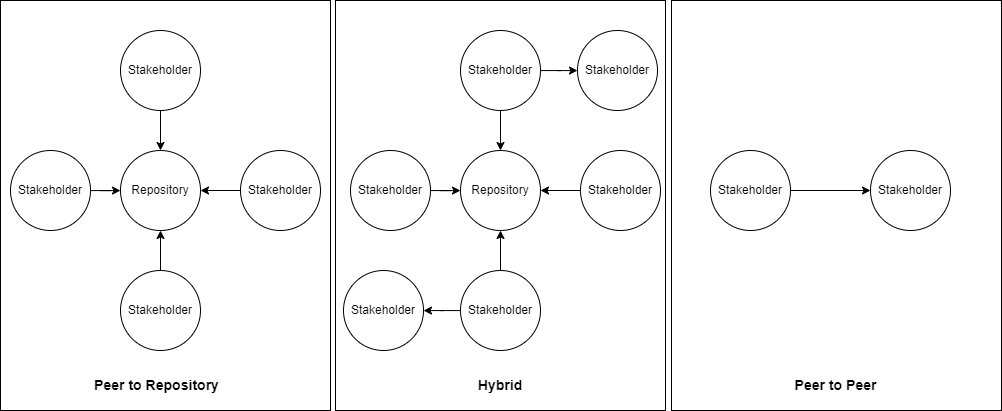
\includegraphics[width=\textwidth]{sharing_models}
    \caption{CTI Sharing Models}
    \label{fig:sharing-models}
\end{figure}

CTI sharing can be either peer-to-peer, peer-to-hub (i.e. Repository), or a combination of the two (Figure \ref{fig:sharing-models}). Traditional exchange of CTI between two organizations is an example of a peer-to-peer sharing. In the peer-to-hub, a hub or repository is used to collect and distribute data. If the repository is openly accessible to anyone, it is called open source CTI sharing. Jesus et al. \cite{jesus_sharing_2023} investigated the state of the art of the open source CTI sharing. They found the barriers that have prevented the formation of any widely used open source CTI platform. 
The barriers mentioned are 1) Legal and regulatory (e.g. GDPR or intellectual property) 2) Interoperability (e.g. different formats) 3) Usefulness and return 4) Market factors (e.g. losing reputation, free-riding) 5) Trust in peers and adversarial usage 6) Confidentiality risks.

After studying these barriers, as well as some technical gaps, they present a confidentiality and privacy analysis of sharing a large sample data set of CTI, to make the claim that it is possible to manage risks of sharing using simple techniques like sanitization. Finally, they propose a set of requirements and a reference architecture for an open source CTI sharing platform. 


\subsection{Current Data Space Initiatives}
There are several initiatives that are working to create a standard for data spaces. The most prominent ones are International Data Spaces (IDS) and Gaia-X. In this section, we will review these two initiatives and compare them.

\paragraph{IDSA}

The International Data Spaces (IDS) is an initiative with the goal of creating a standard for a distributed software architecture for data exchange with sovereignty. It was launched in 2015 as a Fraunhofer research project funded by the German Federal Ministry for Education and Research \cite{otto_evolution_2022}. Shortly after that, in 2016, the IDS Association (IDSA) was founded as a non-profit organization to continue the research. It resulted in definition of the IDS Reference Architecture Model (IDS RAM). The IDS RAM is the description of IDS components and their interactions without being technology specific \cite{otto_evolution_2022}. IDS RAM allows anyone to implement the IDS compliant components using any technology. The IDSA also provides a reference implementation of different IDS components called IDS Testbed \footnote{https://internationaldataspaces.org/offers/reference-testbed/}. 

\subparagraph{IDS RAM}
IDS RAM defines the following components:
Connector, Identity Provider, IDS Broker, Clearing House, IDS Apps, App Store, Vocabulary Provider \cite{pettenpohl_international_2022}.
% \begin{itemize}
%     \item Connector: The connector is the interface between the IDS ecosystem and the data source. It is responsible for the data exchange and the enforcement of the usage control policies as well as authentication.
%     \item Identity Provider: authentication service managing identity information
%     \item IDS Broker: Manages the metadata (description and usage policies)
%     \item Clearing House: Audits the data exchange and manages the payment
%     \item IDS Apps: Process the exchanged data. Deployed within Connector.
%     \item App Store: Provides IDS apps
%     \item Vocabulary Provider: Offers vocabularies to describe and annotate data
% \end{itemize}
Furthermore, it conceptualizes the following roles for the participants:
Data Owner, Data Provider, Data Consumer, Data User, App Provider
\cite{pettenpohl_international_2022}.
% \begin{itemize}
%     \item Data Owner: Controls the data and defines usage policies and payment model.
%     \item Data Provider: Provides the data to the IDS ecosystem with respect to the policies defined by the data owner.
%     \item Data Consumer: Same as data provider but consumes the data.
%     \item Data User: Same as data owner but uses the data.
%     \item App Provider
%     \item ...
% \end{itemize}
% Usage Control:
Also, it defines the standards and procedures to ensure data sovereignty. It uses usage control to enforce the usage policies defined by the data owner. It uses the following components to do so: Usage Control Policy Management Point (UC PMP), Usage Control Policy Decision Point (UC PDP), Usage Control Policy Enforcement Point (UC PEP) \cite{otto_evolution_2022}.
The policies are defined in a machine-readable format which is an extension of the Open Digital Rights Language (ODRL) \cite{eitel_usage_2021}. These policies should be mapped to a specific policy language supported by the tool that enforces them. IDSA RAM mentions the following policy enforcement tools: MYDATA \footnote{https://www.dataspaces.fraunhofer.de/en/software/usage-control/mydata.html}, LUCON \footnote{https://www.dataspaces.fraunhofer.de/en/software/usage-control/lucon.html}, D° \footnote{https://www.dataspaces.fraunhofer.de/en/software/usage-control/d.html}. 
% Certification:
% TODO: Add more details about the certification process


\paragraph{Gaia-X}

Gaia-X is an initiative, launched in 2019, that aims to foster creation of an infrastructure that allows for free and easy exchange of data and services between organizations and evade the vendor lock-in imposed by current proprietary cloud and service providers. To do so, regulations and technical specifications that are based on European values, applicable to any existing cloud and edge technology stack are going to be defined. The goal is to bring transparency, controllability, portability and interoperability across data and services. By facilitating data collection and sharing between organizations, a vibrant data ecosystem across Europe and beyond could evolve. Gaia-X Association deliverables include federation services, common policy rules and an architecture of standards. Federation services can be utilized by the ecosystem participants to achieve a global interoperability, compliance and effortless set up. This includes, “Identity and Trust”, “Federated Catalog” and “Data Exchange services”. \cite{otto_role_2022}
% AISBL: Gaia-X Association
% Nodes, Services (Any cloud service), Service Instances (A service running on a node) and Data Assets (a data set on a node)
% Participants: Organizations and individuals that are part of the Gaia-X ecosystem
% Clearing House: Middle man in the exchange checking for compliance

\paragraph{Comparison of IDS and Gaia-X}

% Mapping of Gaia-X to IDS
    % Federated Catalog ~ IDS Broker + Vocabulary Provider + Information Model
    % Identity and Trust ~ IDS Identity Provider + Dynamic Attribute Provisioning Service (DAPS)
    % Gaia X Sovereign Data Exchange ~ IDS Usage Control and Clearing House
    % Gaia X Node ~ IDS Connector

%  Why choose IDSA? 
    % Maturity
    % Open source Reference Implementation
    % Big picture cloud vs. data exchange

% TODO: 
    % IDSA: usage control
    % Gaia-X: Data at rest

In comparison to IDSA, Gaia-X is less mature and still in the development phase whereas IDSA is used in the industry. It focuses on cloud infrastructures and businesses operating within EU, in contrast to IDSA which is more on the technicalities of the sovereign data exchange. Finally, Gaia-X can use IDSA in the data exchange layer \cite{otto_prof_dr_boris_gaia-x_2021}. 


% ---------------------------------------------------------------

\section{Use case and Requirements} % 3 Pages
\label{sec:use-case}

% Scenario
% Requirements
% Constraints

% Two motivations for usage control:
% - Internal: 
% - External: EU-GDPR

% - Confidentiality
% - Security
% - Do we need plausible deniability?
% - Combat against free-riding
% - Trust and reputation

% Some intro about this section
In this section, we will describe the use case and the requirements of the proposed platform. We will also discuss the constraints and limitations of the platform.

\subsection{Overview}
Bazaar can be utilized in several areas. To generalize, any set of organizations that work together to achieve a common goal who fundamentally use IT systems in their operations can benefit from Bazaar. Bazaar can accelerate the process of establishing new sector ISACs and facilitate the activities of existing ones. 
As mentioned in the \ref{sec:ccti}, ISACs' common use cases are critical infrastructures, including, electricity, water, finance, transportation, and healthcare.

To elicit some concrete scenarios where Bazaar can be used, we should narrow our focus on a specific use case. In this work, we will focus on the smart grid use case. Consider a situation where there are several participants representing different organizations active in the energy supply chain. 
The threat landscape they are exposed to is similar, because they are targeted by similar adversaries, and by using same technologies, they share the same vulnerabilities. Therefore, they can benefit from sharing CTI with each other.

A possible threat actor can be an advanced persistent threat (APT) supported by an enemy government, or a gang of experienced cyber criminals intended to disrupt the energy supply by attacking different actors in the supply chain. By doing so, they can reach their goal of causing a blackout, exfiltrating sensitive information, or gaining financial benefits (e.g. ransomware). To this end, they probably use some limited set of tactics, techniques, and procedures (TTP) to attack their victims over and over again. As a result, sharing these TTPs among the participants can help them to be better prepared against these attacks.

Moreover, the participants in the energy sector are required to share information about incidents happened to them with each other and with the national CSIRT. This is required by the NIS2 directive. Therefore, they can use Bazaar to share the required information with each other.

Here, we assume that participants are the security team of the aforementioned organizations, or a managed security service if the organization does not have its own security team. That is because the security team is the entity responsible for handling the CTI, and we do not consider other types of security information (e.g. logs) in this work.

To maximize the benefits of information sharing, we extend the possible users of Bazaar to include organizations from different countries adhering to different regulations. Example of a challenge that might arise is the GDPR. It limits the transfer of personal data outside the EU. On top of that, language and cultural differences might exist between the participants which will further complicate the trust building and information sharing process. 
As a result, we are dealing with heterogeneous organizations and different levels of trust among the participants, which the platform should be able to handle.


A use case diagram is shown in figure \ref{fig:use-case}.


\begin{figure}[h]
    \centering
    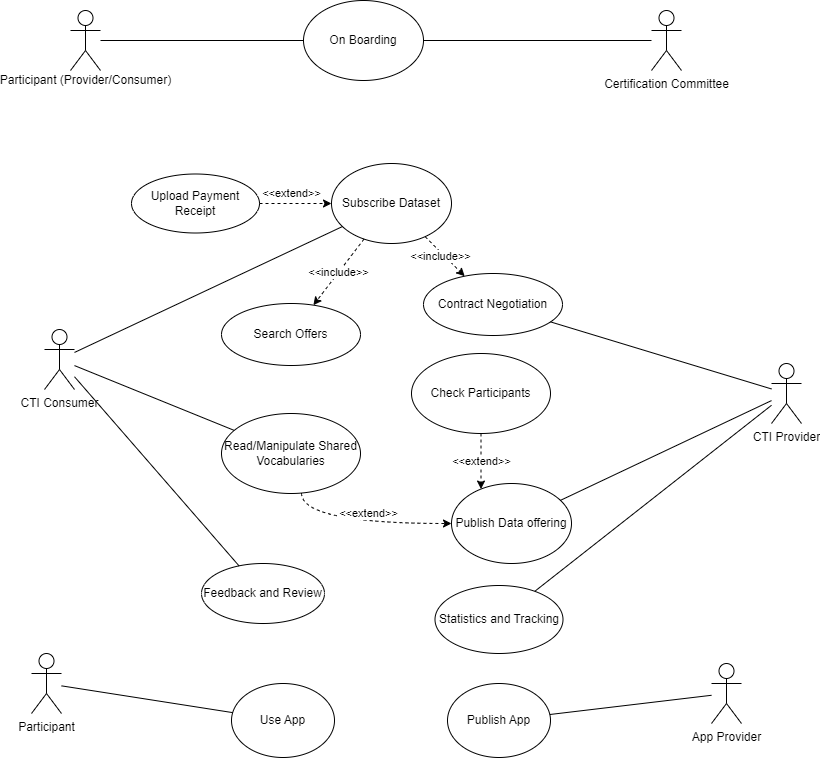
\includegraphics[width=\textwidth]{use_case}
    \caption{Use Case Diagram}
    \label{fig:use-case}
\end{figure}


\subsection{Scenarios}

% Not needed to define use case scenarios using formal templates
% Current level of detail is enough

\paragraph{Scenario 1: Peer to Peer Sharing}
A utility provider (Acme) has found a new malware in their network. They share the related IOC inside Bazaar. However, they set the usage policy to only allow the data to be processed in the Bazaar Connectors located within the EU (to comply with GDPR). They also set the usage policy to only allow the data to be read by the participants that have a certain minimum level on a certain trust metric. Furthermore, Acme does not want to share with competing companies. Therefore, it blacklists identified participants that compete in the same market.


\paragraph{Scenario 2: Paid Service and Rating}

A security organization specialized in selling CTI feeds, wants to use Bazaar to sell its services. It has a set of CTI feeds that it wants to share with its customers. It wants to charge its customers based on the number of IOCs they receive. Customers are also invited to rate the quality of the feeds they receive. This ratings are used by the customers to choose between different feeds.


\paragraph{Scenario 3: Initiation and Explore}

Another organization (Organization B) after having heard of the platform finds it useful. To join the platform, B should pass the necessary certification process.
First, a committee of decision-making community members should accept the request. Then, after technical certification by the platform admins, B is allowed to join. 
At this point, B should be able to connect to the platform. It should be able to search for available data assets, and fetch metadata. It should explore the existing members and their reputation.

\subsetion{Requirements}


% Stake-holders (Actors) and their profile
% - Utility Provider
% - Utility Operator (GO)
% - BSI (in Germany) (?)
% - Gov (CERT, CSIRT, BSI)
% - ISAC
% - SMEs
% - SOC (Different Tiers)
% - MSSP (Managed Security Service Provider)



\section{Conceptual Approach} % 1.5 Pages
\label{sec:conceptual-approach}

% Components and relation to requirements
% Discuss Benefits and limitations
% Compare with existing solutions

\begin{figure}[h]
    \centering
    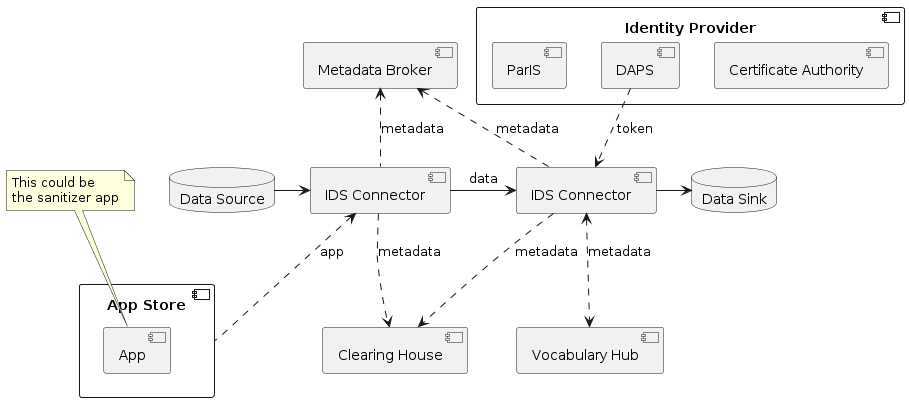
\includegraphics[width=\textwidth]{components}
    \caption{System Architecture Diagram}
    \label{fig:system-architecture}
\end{figure}

Important data space components that are relevant to our use case are listed below. The descriptions fully conform to the IDSA RAM 4.0 \cite{otto_ids_2019}.
\begin{itemize}
    \item Connector: It is the primary component involved in the data exchange acting either as data provider or consumer. Not only it performs the actual data exchange but also the enforcement of the usage control policies as well as authentication. It can be operated on-premises or in a cloud environment. It will run the IDS Apps that do process the data among other things (more on that later). It uses application container management technology to isolate data apps and core functionalities.
    \item IDS Broker: The IDS Metadata Broker is an IDS Connector, which contains an endpoint for the registration, publication, maintenance, and query of Self-Descriptions. Self-Descriptions encapsulate information about Connectors, their managing participant, the offered data assets, and the respective usage conditions. In a sense, the IDS Broker is like a phonebook.
    \item Identity Provider: This is the component serving as Identity and Access Management (IAM). It's responsible for assigning identities to participants, verifying identity claims and granting access based on identities. It comprises three components: 
        \begin{itemize}
            \item CAs: One or multiple certificate authorities are responsible for issuing certificates to participants upon request. They are also responsible for revoking certificates. They are the trust anchors by which all other components can be verified.
            \item Dynamic Attribute Provisioning Service (DAPS): It complements the certificates issued by CAs with more volatile attributes in form of tokens. Connectors can request Dynamic Attribute Tokens (DATs) from DAPS to prove their attributes to other components.
            \item Participant Information Service (ParIS):  It provides business-related information about participants in the IDS that have been checked by the Support Organization. Similar to the way Broker provides metadata about data assets, ParIS provides metadata about participants.
        \end{itemize}
    \item Clearing House: It is a trusted third party in the data exchange that logs all the required information about clearing, billing, and usage control. It keeps track of the payment information and also usage information to help verify the compliance with the usage policies.
    \item IDS Apps: These are re-usable software components that can be deployed inside the IDS Connector. They are mainly used to transform or analyze data. However, they can also be used to connect to enterprise services, or to allow the connector to be controlled by external systems. Data apps can be chained and bundled.
    \item App Store: As the name suggests, it is a marketplace for IDS Apps. It contains endpoints to publish, search, and download IDS Apps. It is a Connector on its own, so it should pass the IDS certification criteria and provide a self-description.
    \item Vocabulary Provider: To facilitate cooperation of different IDS components, a common vocabulary is required. The vocabulary provider enables the participants to define and publish their own vocabularies. Vocabularies typically follow the RDF standard. An example usage is to reference an RDF URI in the Self-Description of a data asset.
\end{itemize}

Apart from the components described by the IDS RAM, there are other components that are not part of the IDS RAM but are relevant to our use case. These components are described below.

\begin{itemize}
    \item Sanitization App: This is an IDS App that is responsible for sanitizing the data. It is deployed inside the IDS Connector. It is responsible for removing the sensitive information from the data before it is shared with other participants. IDS App is suitable for this task because dealing with sensitive data requires a high level of trust. Apps are certified and verified by the App Store. Furthermore, they are executed within the Connector, so they have access to the data before it is shared with other participants. This is important because it prevents the data from being leaked before it is sanitized. 
\end{itemize}

\section{Realization / Implementation} % 1 Page
\label{sec:realization}
% Which technology and tools you use?
% Architecture
% - Which parts will you implement yourself, and which part you copy?
%     - IDS Testbed
%     - 

% - How they fit with dataspace components?

\subsection*{IDS Connector}
The IDS Association publishes a monthly report of the current state of all the data connectors used for exchange of data, not limited to the IDS compliant connectors.
 Dam et al. \cite{dam_survey_2023} investigated this report and published a survey in September 2023. They found that only 4 connectors have their source code available on a public repository: 1) IDS Dataspace Connector (DSC) by sovity, Eclipse Dataspace Connector (EDC), the TRUsted Engineering (TRUE) Connector, and the Trusted Connector by Fraunhofer AISEC.

In addition to that, I found two more: First, IDS Integration Toolbox by Open Logistics Foundation which is a wrapper around the DSC. Second, TNO Security Gateway (TSG) initially developed by TNO which has implementations for many IDS components. It is used in Smart Connected Supplier Network (SCSN) data space and has a documentation.
However, it has no stars on gitlab.

The overview of different conenctors is shown in table \ref{tab:connectors}.

\begin{table}[ht]
    \label{tab:connectors}
    \centering
    \begin{tabular}{| c c c c c c|}
    \hline
    \textbf{Name} & \textbf{Created} & \textbf{Stars} & \textbf{Commits} & \textbf{Last Release} & \textbf{Hosted} \\
    \hline
    \hline
    DSC & 07.10.2020 & 27[+101] & 2600 & 10.22 & \href{https://github.com/International-Data-Spaces-Association/DataspaceConnector}{Github} \\
    \hline
    EDC & 13.01.2021 & 202 & 1817 & 10.23 & \href{https://github.com/eclipse-edc/Connector}{Github} \\
    \hline
    TRUE & 30.10.2020 & 19 & 122 & 08.23 & \href{https://github.com/Engineering-Research-and-Development/true-connector}{Github} \\
    \hline
    Trusted & 05.09.2017 & 43 & 2221 & 02.23 & \href{https://github.com/Fraunhofer-AISEC/trusted-connector}{Github} \\ 
    \hline
    Toolbox & 31.03.2022 & 3 & 172 & 04.23 & \href{https://git.openlogisticsfoundation.org/silicon-economy/base/ids/ids-integration-toolbox}{Self-Hosted} \\
    \hline
    TSG & 12.05.2021 & 0 & 243 & 08.23 & \href{https://gitlab.com/tno-tsg}{Gitlab} \\
    \hline
    \end{tabular}
    \caption{Available IDS Connectors}
\end{table}

Most number of stars and most recent release being a deciding factor, I will choose EDC to base my implementation on.

\subsection*{IDS Testbed}
The IDS association defines Minimum Viable Data Space (MVDS) as the minimum set of components that provide the ability to do secure and sovereign data exchange. They specify the required components as follows: Two Connectors (a data provider and a consumer), an Identity Provider (Dynamic Attribute Provisioning Service, Certificate Authority). IDSA has published an open-source project, \href{https://github.com/International-Data-Spaces-Association/IDS-testbed}{IDS Testbed}, that contains instructions to install and orchestrate these set of minimum components. It references open-source implementations of these components, see table \ref{tab:components} to find source code of these components.

\begin{table}[h]
    \label{tab:components}
    \centering
    \begin{tabular}{|c|c|c|c|}
    \hline
    \textbf{Component} & \textbf{Source Code} & \textbf{Version} & \textbf{Language} \\
    \hline
    IDS Testbed & \href{https://github.com/International-Data-Spaces-Association/IDS-testbed}{Testbed Git} & 1.0 & Docker-Compose \\
    \hline
    Connector & \href{https://github.com/International-Data-Spaces-Association/DataspaceConnector/tree/v8.0.2}{Connector Git} & 8.0.2 & Java \\
    \hline
    Metadata Broker & \href{https://github.com/International-Data-Spaces-Association/metadata-broker-open-core}{Broker Git} & 5.0.3 & Java \\
    \hline
    DAPS & \href{https://github.com/International-Data-Spaces-Association/omejdn-daps}{DAPS Git} & 1.6.0 & Ruby \\
    \hline
    Certificate Authority & \href{https://github.com/International-Data-Spaces-Association/IDS-testbed/tree/master/CertificateAuthority}{Testbed Git} & --- & Python \\
    \hline
    App Store & \href{https://github.com/International-Data-Spaces-Association/IDS-AppStore}{App Store Git} & 3.0.0 & Java \\
    \hline
    \end{tabular}
    \caption{Necessary Components}
\end{table}

In addition to the aforementioned components, some new ones need to be implemented from scratch: App Store, ParIS, Clearing House, Vocabulary Hub. Of course, the required IDS Apps should be implemented, which includes, the Sanitization App. 
For the App Store there is a published project (\href{https://github.com/International-Data-Spaces-Association/IDS-AppStore}{App Store Git}) which is not included in the testbed and might not be fully functional.

\subsection*{Usage Policies}
To describe usage policies IDS defines its own Usage Control Language which is an extension of Open Digital Rights Language (ODRL). It is a machine readable format which is technology agnostic. There are multiple mechanism to enforce these policies automatically. The position paper on IDS Usage Control \cite{eitel_usage_2021} lists the following mechanisms: MYDATA Control Technologies, Logic based Usage Control (LUCON), and Degree (D°). According to the paper, MYDATA Control Technologies is the most mature and comprehensive. It is also the only one that is implemented in the IDS Testbed. Therefore, I will use MYDATA Control Technologies to enforce the usage policies. The usage control is enforced in the IDS Connector possibly using a separate application container. It comprises three different components: PMP, manages policies and creating them based on some templates, PDP, evaluates the policies and decides whether to allow or deny the request, and PEP, enforces the decision made by PDP. The overview of the components is shown in figure \ref{fig:connector}.

\begin{figure}[h]
    \centering
    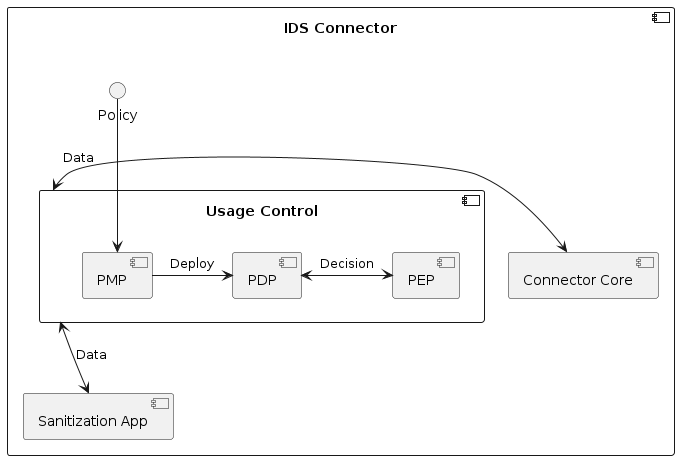
\includegraphics[width=\textwidth]{connector}
    \caption{Connector Overview}
    \label{fig:connector}
\end{figure}


\subsection*{Sanitization App}
Removing all sensitive data from CTI in general can be a difficult task. There are different CTI formats and each format has its own structure. Furthermore, deciding whether a value contains confidential information or not is not straight-forward. Even a sophisticated machine learning approach requires a lot of data with different types of confidential information to be trained on. Therefore, I will focus on creating a base sanitization app that is easily extensible to detect more sensitive data. To start, it should support sanitizing JSON based CTI formats, and a configurable set of regex rules to detect sensitive data. Refining this app to support more formats and more sophisticated detection mechanisms is out of scope of this thesis.

\section{Evaluation} % 0.5 Page
\label{sec:evaluation}
% Methodology and Metrics
% Test scenario

% - How to gather (CTI) data?
% - Metrics for evaluating the privacy? (e.g. entropy)
% - The steps of the scenario and the expected results
% - How to measure the performance?

My contribution being design of a sharing platform for CTI data, the evaluation should measure the effectiveness of the sharing platform. The problem is that according to my research, there is no benchmark available and no defined metrics to this aim. Having no baseline to compare against, it seems hard to reach an objective evaluation. Furthermore, many performance metrics depend on the implementation, infrastructure, and the details of the scenario. Since, my main contribution is the design of the platform, not the implementation, some metrics can be misleading. 

However, several options can be thought of. First, by focusing on the main effect of using data spaces for data sharing, which is the addition of usage control and changing the data flow, one can define a few specific metrics. Having defined some usage case scenarios and a sample implementation, we can measure for example the following metrics: 
\begin{itemize}
    \item Number of unnecessary participants that should have access to the data.
    \item The difficulty of changing the usage policies.
    \item How difficult it is to revoke access to the data.
    \item Variety of types of usage policies that are enforceable.
    \item How many scenarios are significantly improved using our approach.
\end{itemize}

The above-mentioned items might be subjective and change by modifying the chosen scenarios, but investigating it can provide some insights into the effectiveness of the data spaces.

Another approach which can sound more objective is to design a survey. It should use some standard templates to be comparable. The survey should be conducted on a group of experts in the field of CTI sharing after presenting them our approach. The survey should be designed to measure the effectiveness of our design in terms of privacy and security. Ideally, 10 to 20 experts should be interviewed. There is a risk of not having enough experts available. In that case, we fall back to the first approach.


\section{Timeline / Milestones / Project Plan} % 0.75 Page
\label{sec:timeline}

TODO

\newpage


\bibliography{References} 
\bibliographystyle{ieeetr}

\end{document}
